\chapter{Quality Measures}\label{quality-measures}

Visual Test
Strutural Test
Report Tool
Coding Standards

\section{Testing}\label{testing}

The osm2vectortiles ecosystem is quite diverse with a big collection of small tools that all work together which makes testing really complex.

\subsection{Integration Test}

In Travis CI\cite{pm_5_travis-ci.org_2015}  the entire workflow was completed for a small data sample on each commit.
Because the entire workflow is configured with Docker Compose \cite{pm_6_docs.docker.com_2015} the CI server had to execute all import steps in serial order. This is a straightforward way to check if all components work together correctly
and although it is a simple setup it has helped tremendously during project development, catching bugs
like missing tables or SQL typos.

\begin{yamlcode}
script:
  # Test import
  - docker-compose up -d postgis
  - sleep 10
  - docker-compose run import-external
  - docker-compose run import-osm
  - docker-compose run import-sql
  # Test export
  - docker-compose run export
  # Test changed tiles
  - docker-compose run update-osm-diff
  - docker-compose run import-osm-diff
  - docker-compose run changed-tiles
\end{yamlcode}

\subsection{Visual Testing}

\begin{figure}[H]
  \centering
  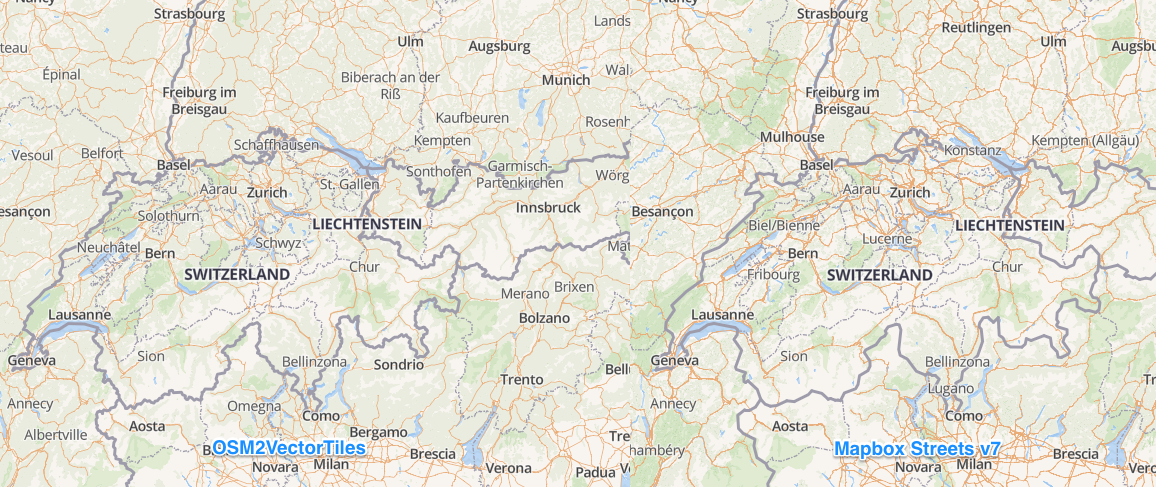
\includegraphics[width=1.0\textwidth]{images/visual_compare}
  \caption{Visual Compare Tool}
  \label{visual_compare} 
\end{figure}

\section{Guidelines}\label{guidelines}
To have homogeneous software the contributors have settled on common guidelines in the beginning of the project.

\subsection{Releases}
Semantic versioning \cite{pm_7_preston-werner_2015} should be used for releases.
At the end of each milestone a new release will be created.
\newpage

\subsection{Git}\label{git}
\paragraph{Commit Messages}
The seven rules of great git commit
messages\cite{pm_8_chris.beams.io_2015} should be used.

\paragraph{Rewriting}
Git history should be kept clean and therefore local branches should be
squashed meaningfully.

\paragraph{Pulling}
To avoid unnecessary merge messages one should always use the
\texttt{-\/-rebase} parameter.

\subsection{Workflow}\label{git-workflow}
The Feature Branch Workflow\cite{pm_9_atlassian_git_tutorial_2015} should be used. Every project member has a local repository with a copy of the remote
repository. For each feature ticket in GitHub a separate branch
will be created. Once a ticket has been completed a pull request will be
created and needs to be merged into the \texttt{master} branch by an other 

\subsection{Coding Standards}

\paragraph{Bash} Bash was used for the Docker image entrypoints and follow
the rules of Defensive Bash Programming \cite{pm_10_lavi_2012}.

\paragraph{Python} Python code should stay PEP-8\cite{pm_11_python.org_2015} compliant and write idiomatic Python code according to PEP-20\cite{pm_12_python.org_2015}.

\paragraph{JavaScript} The JavaScript code is checked using ESLint\cite{pm_13_eslint.org_2015}

\paragraph{SQL} The PostgreSQL code is using upper case for the key words. Apart from nice formatted SQL code and functions should be used
to keep the queries DRY\cite{pm_14_wikipedia_2015}.

\paragraph{Dockerfile} Dockerfiles follow the best practices\cite{pm_15_docs.docker.com_2015} defined by Docker.
